By employing the data collection and analysis methods outlined 
below, this study aims to comprehensively explore the protein 
sequences of plants and their adaptive relationships based 
on KOGs. The integration of bioinformatics tools, hierarchical 
classification, and statistical analyses offers novel insights 
into plant evolution and functional adaptations.


\subsection{Data Collection and Selection}
\label{sec:method.data}

A comprehensive dataset of protein sequences from diverse plants 
is retrieved from the PhytozomeV13 Database~\citep{goodstein2011}.
This dataset consists of 114 proteomes, including 100 
Angiosperms (29 Monocots, 70 Eudicots, and \emph{Amborella 
trichopoda}), 10 Algae (9 \emph{Chlorophyta} and 1 
\emph{Rhodophyta}), and 4 other species: \emph{Marchantia 
polymorpha}, \emph{Physcomitrella patens}, \emph{Selaginella 
moellendorffii}, and \emph{Sphagnum fallax}. Careful selection 
ensured representation across various plant families and a 
broad taxonomic range. The complete list with the information 
of the species can be found in the Supplementary material. The 
corresponding phylogenetic tree is shown in 
Figure~\ref{fig:taxa}, which is created from the NCBI Taxonomy 
Browser and constructed using the online tool Interactive 
Tree Of Life~\citep{letunic2021}.

\begin{figure}[htp]
\centering
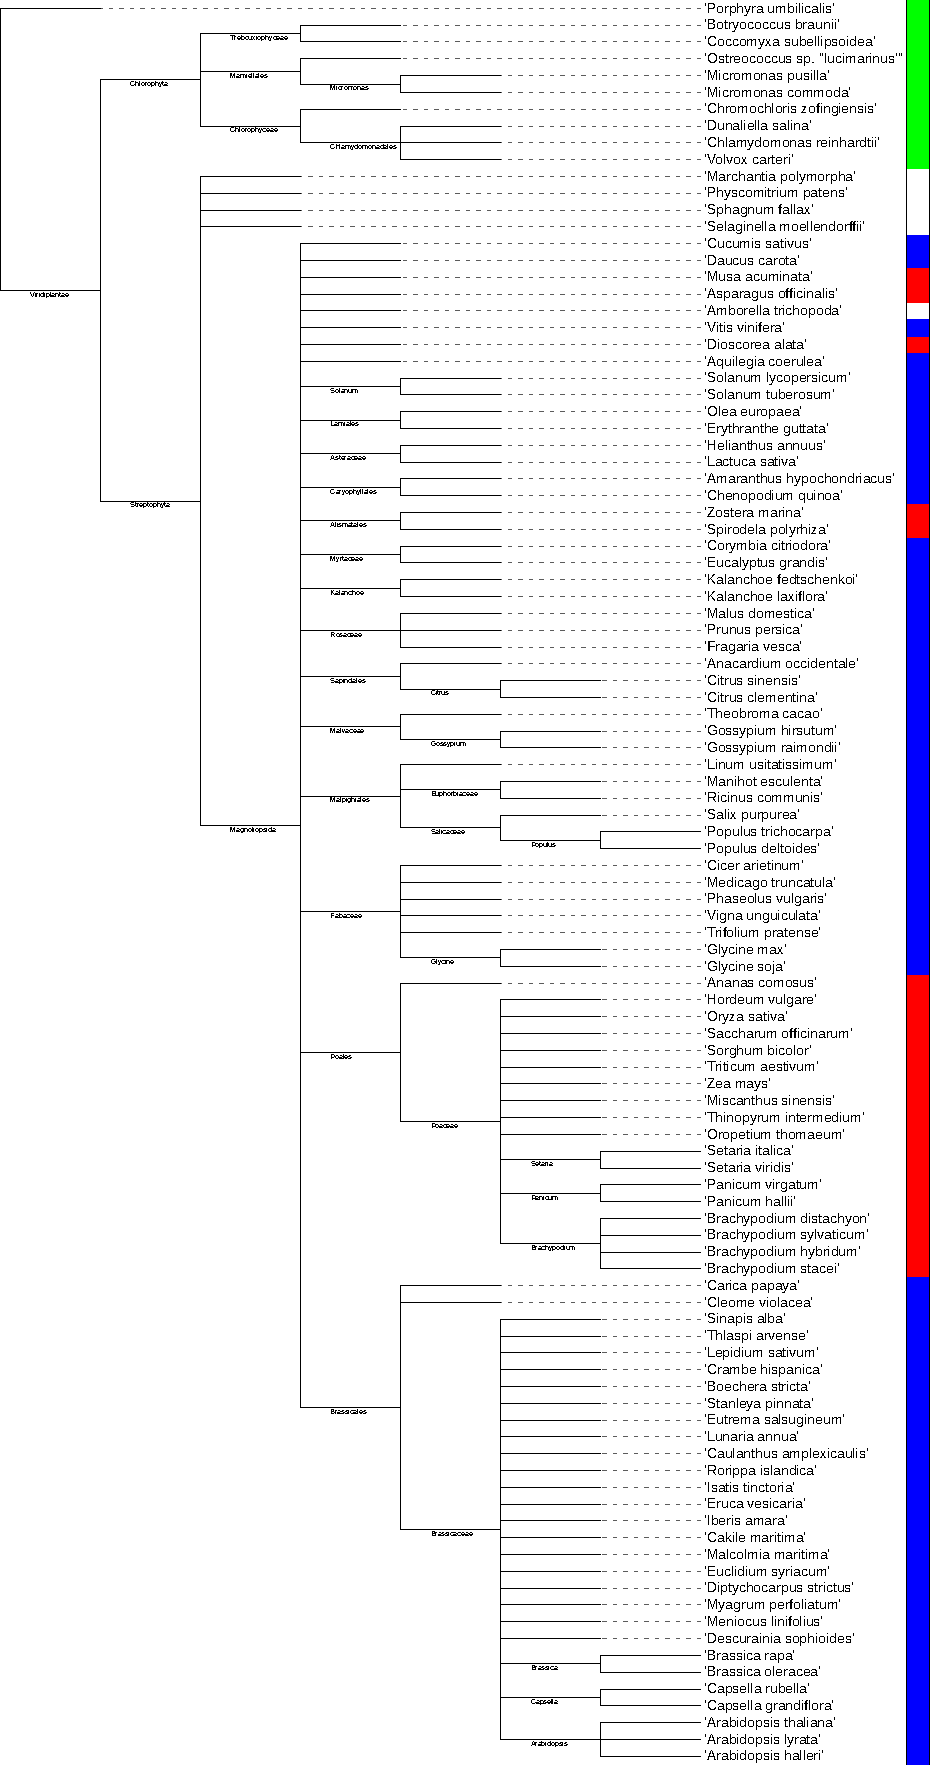
\includegraphics[width=0.9\textwidth]{figures/Taxa}
\caption{Taxonomy tree of the plant species of this study. 
The color tag corresponds to each biological category: 
Eudicots in blue, Monocots in red, Algae in Green and 
Other in white.
}
\label{fig:taxa}
\end{figure}


\subsection{Eukaryotic Orthologous Groups (KOGs) Analysis}
\label{sec:method.kog}

The Eukaryotic Orthologous Groups (KOGs) database by 
\cite{tatusov2003} is used to analyze the collected protein 
sequences. A sequence alignment approach (BLASTP) mapped the 
selected protein sequences to the corresponding KOGs, 
identifying orthologous groups and conserved 
domains~\citep{camacho2009}. Only BLASTP matches with an 
identity greater than or equal to 95\% were considered.

Subsequently, annotations were transferred to all species, 
and the frequency of each annotation was assessed as the 
number of proteins in each transferred category (e.g., K - 
Transcription). Protein counts were scaled relative to the 
total number of proteins in each organism, enabling a 
fair comparison despite varying annotation coverage after 
BLASTP alignment.


\subsection{Hierarchical Classification based on KOG Counts}
\label{sec:method.hierarchy}

To gain insights into the evolutionary relationships among 
the studied plant species, a hierarchical classification 
system is used based on KOG counts of annotated proteins. 
The normalized frequency of each annotation serves as a 
26-dimensional vector representation for each species. Using 
the \emph{linkage} algorithm with parameters set to "ward" 
for method and "euclidean" for metric from the scipy library 
in Python, a hierarchical organization of plant species with 
similar KOG profiles is obtained at different taxonomic 
levels. The linkage approach provided a visual representation 
of the relationships between taxa, offering a hierarchical 
perspective of plant evolution. Additional vignettes were 
included in the graphical representation to apply biological 
categories to plants: Monocot, Eudicot, Alga, or Other. 
For simplicity, \emph{Amborella trichopoda} is included in 
the Other category for simplicity.


\subsection{Comparison of Gene Ontology and Phytozome}
\label{sec:method.compare}

To validate the KOG-based classification of Phytozome proteomes 
and explore the functional implications of identified 
orthologous groups, a 
comparison with information from the Gene Ontology (GO) 
database was performed~\citep{ashburner2000,consortium2023}.
Namely, the annotated proteomes of GO are retrieved and the 
same procedure of KOG annotation transfer is performed on them.

The results obtained with Phytozome are summarized by 
computing the mean and standard deviation for each KOG 
category among all species and each phylogenetic category. 
Similarly, functional annotations from the GO database are 
transferred to each organism using BLASTP, and frequency 
counts for those annotations are computed. Besides, an 
additional computation is performed on the frequency counts, 
from now on addressed as normalized count: the frequencies 
for a proteome were scaled to add up to 1. Note that this 
values are different from the results of the previous 
scaling procedure, due to the vast amount of proteins 
without a representative ortholog in the model proteome 
of KOG. Furthermore, the normalized values for each 
biological category are computed for the Phytozome data and
compared among them and against the global distribution.

Through statistical analyses and correlation studies, the 
concordance between the KOG-based classification on Phytozome 
and GO was assessed. This comparison allowed for 
evaluation of the consistency and reliability of the 
hierarchical classification and provided insights into the 
functional relevance of the identified protein groups.
